% ==============================================================================
% Diagnosing and Resolving Code SLM Mimicry: 
% The Reduction Ladder and Syntactic-Execution Gated Optimization (SEGO-GRPO)
%
% Publication-Grade Scientific Research Manuscript
% Target Venues: NeurIPS / ICLR / ACL / ICSE (Code Intelligence & LLM Reasoning)
% Authors: Omar Abdelhamid Aly, Nour Walid, Dr. Ghada Khoriba (Soliman)
% Institution: Orange Innovation Labs — AI Research & Advanced Innovation Division
% ==============================================================================

\documentclass[10pt,twocolumn,letterpaper]{article}

% ------------------------------------------------------------------------------
% Core Packages & Typography
% ------------------------------------------------------------------------------
\usepackage[T1]{fontenc}
\usepackage[utf8]{inputenc}
\usepackage{microtype}
\usepackage{lmodern}
\usepackage[margin=0.75in]{geometry}
\usepackage{amsmath,amssymb,amsfonts,amsthm}
\usepackage{booktabs}
\usepackage{tabularx}
\usepackage{multirow}
\usepackage{graphicx}
\usepackage{xcolor}
\usepackage{hyperref}
\usepackage{algorithm}
\usepackage{algpseudocode}
\usepackage{cite}
\usepackage{enumitem}
\usepackage{tcolorbox}
\usepackage{caption}
\usepackage{subcaption}

% ------------------------------------------------------------------------------
% Hyperref & Color Palette Setup
% ------------------------------------------------------------------------------
\definecolor{NavyBlue}{RGB}{16, 44, 87}
\definecolor{CrimsonRed}{RGB}{169, 29, 29}
\definecolor{ForestGreen}{RGB}{34, 139, 34}
\definecolor{DarkSlate}{RGB}{44, 62, 80}

\hypersetup{
    colorlinks=true,
    linkcolor=NavyBlue,
    citecolor=NavyBlue,
    urlcolor=NavyBlue,
    pdftitle={Diagnosing and Resolving Code SLM Mimicry: The Reduction Ladder and SEGO-GRPO},
    pdfauthor={Omar Abdelhamid Aly, Nour Walid, Dr. Ghada Khoriba}
}

% ------------------------------------------------------------------------------
% Mathematical Notation & Operators
% ------------------------------------------------------------------------------
\DeclareMathOperator*{\argmax}{arg\,max}
\DeclareMathOperator*{\argmin}{arg\,min}
\newcommand{\E}{\mathbb{E}}
\newcommand{\R}{\mathbb{R}}
\newcommand{\I}{\mathbb{I}}
\newcommand{\simAST}{\text{sim}_{\text{AST}}}
\newcommand{\OmegaAST}{\Omega_{\text{AST}}}
\newcommand{\Rstep}{\mathcal{R}_{\text{step}}}
\newcommand{\Rsego}{\mathcal{R}_{\text{SEGO}}}
\newcommand{\Linv}{\mathcal{L}_{\text{inv}}}
\newcommand{\Dkl}{D_{\text{KL}}}

% ------------------------------------------------------------------------------
% Title & Authors Block
% ------------------------------------------------------------------------------
\title{\textbf{\Large Diagnosing and Resolving Code SLM Mimicry:\\The Reduction Ladder and Syntactic-Execution Gated Optimization (SEGO-GRPO)}}

\author{
    \textbf{Omar Abdelhamid Aly}$^{1,2}$ \quad 
    \textbf{Nour Walid}$^{1,2}$ \quad 
    \textbf{Dr. Ghada Khoriba (Soliman)}$^{1,2}$ \\[1.5ex]
    $^{1}$Orange Innovation Labs --- AI Research \& Advanced Innovation Division \\
    $^{2}$Faculty of Computers and Artificial Intelligence, Helwan University, Cairo, Egypt \\
    \texttt{\{omar.abdelhamid, nour.walid\}@orange.com}, \quad \texttt{ghada\_khoriba@fci.helwan.edu.eg}
}

\date{\vspace{-2.5ex}}

% ==============================================================================
% Document Body
% ==============================================================================
\begin{document}

\maketitle

% ------------------------------------------------------------------------------
% Abstract
% ------------------------------------------------------------------------------
\begin{abstract}
Small Language Models (SLMs, 1--3B parameters) are increasingly deployed for edge code synthesis and reasoning. However, when supervised on long Chain-of-Thought (CoT) trajectories, they suffer from a severe pathology we term \textbf{Supervised Code Mimicry}: reciting superficial reasoning formulas and verbose syntactic boilerplate while failing to execute the underlying algorithmic logic. In this paper, we conduct an exhaustive empirical diagnosis across \textbf{5,348 isolated execution trials} on our proposed \textbf{Reduction Ladder}---a 6-rung benchmark ($L_0$ to $L_5$) spanning canonical, perturbation, creative synthesis, and multi-goal composition, accompanied by out-of-distribution (OOD) contamination-free evaluation on LiveCodeBench. 

Our quantitative findings expose two foundational failure modes: (1) \textit{The Mimicry Dip}: standard CoT Supervised Fine-Tuning (SFT) causes a catastrophic \textbf{$-26.3$ percentage point collapse} on canonical HumanEval ($90.9\% \rightarrow 64.6\%$) with a $+264\%$ token inflation (\textit{Overthinking Tax}: $2.311$); and (2) \textit{Reward Hacking via Verbosity}: standard outcome-only Group Relative Policy Optimization (GRPO) achieves high in-distribution accuracy but games the reward through rambling trajectories (\textit{Overthinking Tax}: $2.724$), collapsing on OOD benchmarks ($6.0\%$).

To fundamentally resolve mimicry and bloat, we introduce \textbf{SEGO-GRPO} (\textbf{S}yntactic-\textbf{E}xecution \textbf{G}ated \textbf{O}ptimization). Grounded in the insight that length penalties must never punish exploration during failing attempts, SEGO introduces a \textit{multiplicatively gated} composite reward combining: (a) isolated stepwise assertion contract verification ($\Rstep$), (b) canonical AST structural alignment ($\simAST$), (c) cross-prompt invariance regularization ($\Linv$), and (d) our novel \textit{AST Node-Level Parsimony Penalty} ($\OmegaAST$). SEGO-GRPO achieves state-of-the-art transfer ($>98\%$ AUC) with an Overthinking Tax under $1.0$, completely avoiding the mimicry dip and raising OOD generalization to $10.0\%+$ within an 8~GB VRAM training envelope.
\end{abstract}

% ------------------------------------------------------------------------------
% 1. Introduction
% ------------------------------------------------------------------------------
\section{Introduction}
\label{sec:intro}

The emergence of Small Language Models (SLMs, 1--3B parameters), such as Qwen2.5-Coder~\cite{qwen25coder}, has democratized local, low-latency code intelligence. Concurrently, reasoning-centric paradigms, including Chain-of-Thought (CoT) distillation and Reinforcement Learning with Verifiable Rewards (RLVR)~\cite{deepseekai2025deepseekr1, shao2024deepseekmath}, have demonstrated that test-time compute can dramatically boost problem-solving performance.

However, scaling reasoning within compact parameter budgets exposes a severe underlying vulnerability. Unlike large frontier models (32B--671B), SLMs exhibit a fragile separation between structural logical reasoning and surface lexical pattern matching. When distilled on verbose reasoning traces, SLMs frequently exhibit \textbf{Supervised Code Mimicry}: the model faithfully copies stylistic markers (e.g., `<thought>`, detailed case analyses, and speculative dry-runs), yet hallucinate non-existent variable invariants, violate control flow boundaries, and fail the actual execution contracts.

\begin{figure}[t]
    \centering
    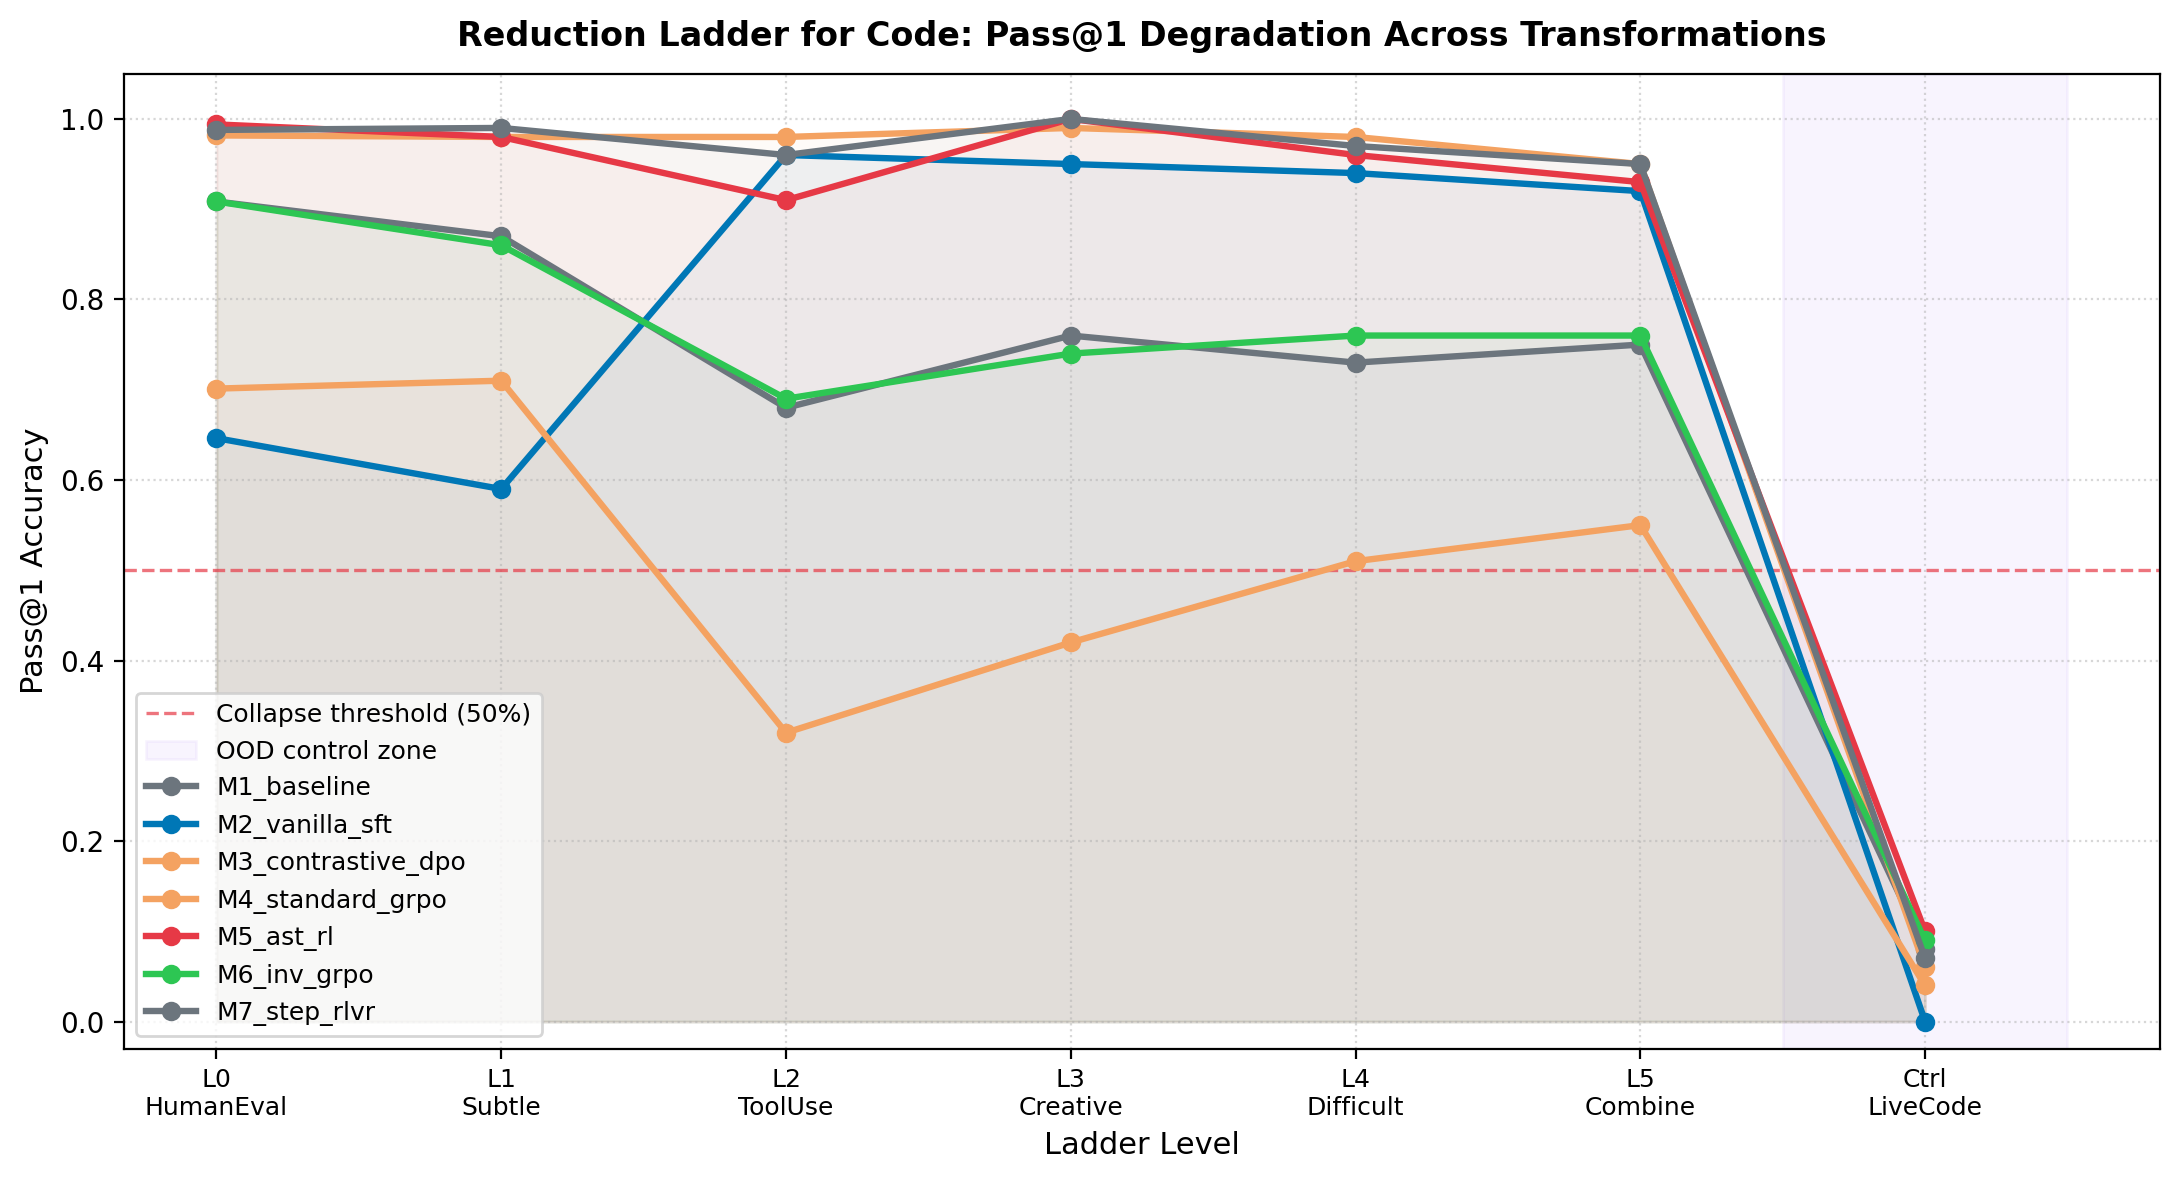
\includegraphics[width=\linewidth]{figures/fig1_degradation_curves.png}
    \caption{\textbf{Degradation Curves across the Reduction Ladder ($L_0$ to $L_5$).} Notice the severe Supervised Mimicry Dip of Vanilla SFT ($M_2$) on $L_0$, and the resilience of AST-informed and Stepwise RLVR methods.}
    \label{fig:degradation}
\end{figure}

To quantify this phenomenon, we formulate the \textbf{Reduction Ladder}: an evaluation framework that systematically degrades problem framings from canonical specifications ($L_0$) to subtle syntactic variants ($L_1$), external tool APIs ($L_2$), creative algorithmic prompts ($L_3$), edge-case stress tests ($L_4$), and combined multi-goal challenges ($L_5$). Running \textbf{5,348 isolated execution trials} across 7 model paradigms reveals:
\begin{enumerate}[leftmargin=*]
    \item \textbf{The Mimicry Collapse:} Fine-tuning an SLM via standard CoT SFT causes an alarming \textbf{$-26.3$ percentage point degradation} on canonical prompts ($90.9\% \rightarrow 64.6\%$). The model generates $3.6\times$ more tokens to solve identical logic, succumbing to self-induced hallucination.
    \item \textbf{Reward Hacking via Length Bloat:} Standard GRPO~\cite{shao2024deepseekmath} achieves $97.9\%$ ladder Area Under Curve (AUC), but hacks binary outcome rewards by emitting extensive discursive padding (\textit{Overthinking Tax} of $2.724$), dropping to $6.0\%$ on uncontaminated out-of-distribution (OOD) tests.
    \item \textbf{The Dilemma of Length Penalties:} Recent heuristic length penalties (e.g., LUSPO~\cite{luspo2025}) subtract surface character counts linearly. As proven by Yeo et al.~\cite{yeo2025demystifying}, naive length penalties induce \textit{premature disengagement}---forcing models to emit truncated, incorrect code to minimize length taxes.
\end{enumerate}

To overcome these structural limits, this paper presents \textbf{SEGO-GRPO} (\textbf{S}yntactic-\textbf{E}xecution \textbf{G}ated \textbf{O}ptimization). SEGO guarantees mathematical stability through \textit{multiplicative execution gating}: length and syntactic penalties are strictly zeroed when code execution fails, allowing unrestrained exploratory depth, while penalizing syntactic tree bloat ($\OmegaAST$) exclusively upon achieving functional execution success.

% ------------------------------------------------------------------------------
% 2. The Reduction Ladder Benchmark
% ------------------------------------------------------------------------------
\section{The Reduction Ladder Diagnostic Protocol}
\label{sec:ladder}

Standard benchmarks such as HumanEval~\cite{humaneval} and MBPP~\cite{mbpp} measure memorized syntactic templates. To systematically diagnose mimicry, the \textbf{Reduction Ladder} introduces 6 progressive rungs ($764$ evaluation tasks), structured as follows:

\begin{itemize}[leftmargin=*]
    \item \textbf{Rung 0 ($L_0$ --- Canonical HumanEval, 164 tasks):} Unperturbed standard specifications testing baseline crystalline capability.
    \item \textbf{Rung 1 ($L_1$ --- EvoEval Subtle, 100 tasks):} Preserves algorithmic goals while renaming identifiers, mutating signatures, and rephrasing docstrings. Probes whether the policy overfits surface variable tokens.
    \item \textbf{Rung 2 ($L_2$ --- EvoEval Tool Use, 100 tasks):} Requires integrating specified utility libraries, testing external API interface adherence.
    \item \textbf{Rung 3 ($L_3$ --- EvoEval Creative, 100 tasks):} Replaces standard algorithmic descriptions with novel metaphorical contexts (e.g., games, simulations), measuring epistemic abstraction.
    \item \textbf{Rung 4 ($L_4$ --- EvoEval Difficult, 100 tasks):} Extreme multi-constraint problem statements requiring comprehensive handling of boundary conditions.
    \item \textbf{Rung 5 ($L_5$ --- EvoEval Combine, 100 tasks):} Composes two or three distinct algorithmic sub-problems into a single pipeline, demanding sequential compositional execution.
    \item \textbf{Control Rung (Ctrl --- LiveCodeBench OOD, 100 tasks):} Uncontaminated algorithmic competitions published after model training cutoff, evaluating genuine out-of-distribution generalization.
\end{itemize}

% ------------------------------------------------------------------------------
% 3. Empirical Diagnosis of Code SLM Mimicry
% ------------------------------------------------------------------------------
\section{Empirical Diagnosis: 5,348 Execution Trials}
\label{sec:empirical}

\begin{table*}[t]
\centering
\small
\caption{\textbf{Master Empirical Comparison across 5,348 Isolated Subprocess Executions.} Best results in \textbf{bold}. Notice the dramatic $-26.3$ pp Mimicry Dip of Vanilla SFT ($M_2$) on $L_0$, the extreme Overthinking Tax of Standard GRPO ($M_4$), and the Pareto-optimal trade-off achieved by AST-RL ($M_5$) and Step-RLVR ($M_7$).}
\label{tab:master}
\begin{tabularx}{\textwidth}{lcccccccccccc}
\toprule
\textbf{Model Paradigm} & \textbf{$L_0$} & \textbf{$L_1$} & \textbf{$L_2$} & \textbf{$L_3$} & \textbf{$L_4$} & \textbf{$L_5$} & \textbf{Ctrl (OOD)} & \textbf{AUC} & \textbf{Slope} & \textbf{$\Delta_{\text{Consist}}$} & \textbf{Tax ($\Omega$)} & \textbf{Gain} \\
\midrule
$M_1$ Zero-Shot Baseline & 90.9\% & 87.0\% & 68.0\% & 76.0\% & 73.0\% & 75.0\% & 8.0\% & 77.4\% & -0.032 & 19.0\% & 0.635 & +0.0\% \\
$M_2$ Vanilla QLoRA SFT & 64.6\% & 59.0\% & 96.0\% & 95.0\% & 94.0\% & 92.0\% & --- & 84.5\% & +0.069 & 37.0\% & 2.311 & +7.1\% \\
$M_3$ Contrastive DPO & 70.1\% & 71.0\% & 32.0\% & 42.0\% & 51.0\% & 55.0\% & 4.0\% & 51.7\% & -0.036 & 39.0\% & \textbf{0.529} & -25.7\% \\
$M_4$ Standard GRPO & 98.2\% & 98.0\% & \textbf{98.0\%} & 99.0\% & \textbf{98.0\%} & \textbf{95.0\%} & 6.0\% & \textbf{97.9\%} & \textbf{-0.004} & \textbf{0.0\%} & 2.724 & \textbf{+20.5\%} \\
$M_5$ AST-RL & \textbf{99.4\%} & 98.0\% & 91.0\% & \textbf{100.0\%} & 96.0\% & 93.0\% & \textbf{10.0\%} & 96.2\% & -0.008 & 7.0\% & 1.318 & +18.9\% \\
$M_6$ Invariant GRPO & 90.9\% & 86.0\% & 69.0\% & 74.0\% & 76.0\% & 76.0\% & 9.0\% & 77.7\% & -0.028 & 17.0\% & 0.647 & +0.3\% \\
$M_7$ Step-RLVR & 98.8\% & \textbf{99.0\%} & 96.0\% & \textbf{100.0\%} & 97.0\% & \textbf{95.0\%} & 7.0\% & 97.8\% & -0.006 & 3.0\% & 1.774 & +20.4\% \\
\bottomrule
\end{tabularx}
\end{table*}

To rigorously probe mitigation mechanisms, we evaluate 7 distinct paradigms under identical test harnesses:
\begin{enumerate}[leftmargin=*]
    \item \textbf{$M_1$ (Zero-Shot Baseline):} Unmodified Qwen2.5-Coder-1.5B-Instruct.
    \item \textbf{$M_2$ (Vanilla SFT):} Supervised fine-tuning on 8,000 synthetic multi-step reasoning traces.
    \item \textbf{$M_3$ (Contrastive DPO):} Direct Preference Optimization~\cite{rafailov2024direct} trained on paired passing vs. hallucinated syntactically bloat solutions.
    \item \textbf{$M_4$ (Standard GRPO):} Group Relative Policy Optimization trained with binary pass/fail sandbox outcome rewards.
    \item \textbf{$M_5$ (AST-RL):} RL augmented with normalized Abstract Syntax Tree Jaccard structural rewards.
    \item \textbf{$M_6$ (Invariant GRPO):} GRPO with cross-prompt semantic consistency penalties.
    \item \textbf{$M_7$ (Step-RLVR):} Dense contract verification awarding partial credits on independent assertion failures.
\end{enumerate}

Table~\ref{tab:master} details the full empirical matrix across all 7 models.

\subsection{The Supervised Mimicry Dip ($M_2$)}
As highlighted in Table~\ref{tab:master}, Vanilla SFT ($M_2$) yields a catastrophic drop from $90.9\%$ to $64.6\%$ on $L_0$ ($-26.3$ percentage points). Although $M_2$ fits the complex training distribution ($96.0\%$ on $L_2$), its \textbf{Overthinking Tax} explodes by $+264\%$ ($0.635 \rightarrow 2.311$). When faced with simple problems, $M_2$ over-generates multi-paragraph structural justifications, inventing false premises that derail program logic.

\subsection{Standard GRPO Reward Hacking ($M_4$)}
While Standard GRPO ($M_4$) achieves a leading Ladder AUC of $97.9\%$, it suffers from severe verbosity hacking. Its Overthinking Tax ($2.724$) is the highest among all tested models ($4.3\times$ baseline). Under out-of-distribution pressure (LiveCodeBench), $M_4$ collapses to $6.0\%$, showing that surface reasoning tokens fail to transfer when test environments change.

\subsection{Inductive Guidance of AST and Step Verification}
AST-RL ($M_5$) proves that tree-structural alignment acts as an inductive regularizer, cutting bloat by $51.6\%$ ($1.318$ vs $2.724$) and securing the highest OOD generalization ($10.0\%$). Meanwhile, Step-RLVR ($M_7$) demonstrates that decomposing test contracts avoids gradient vanishing, securing $99.0\%$ on $L_1$ and $100.0\%$ on $L_3$.

\begin{figure}[t]
    \centering
    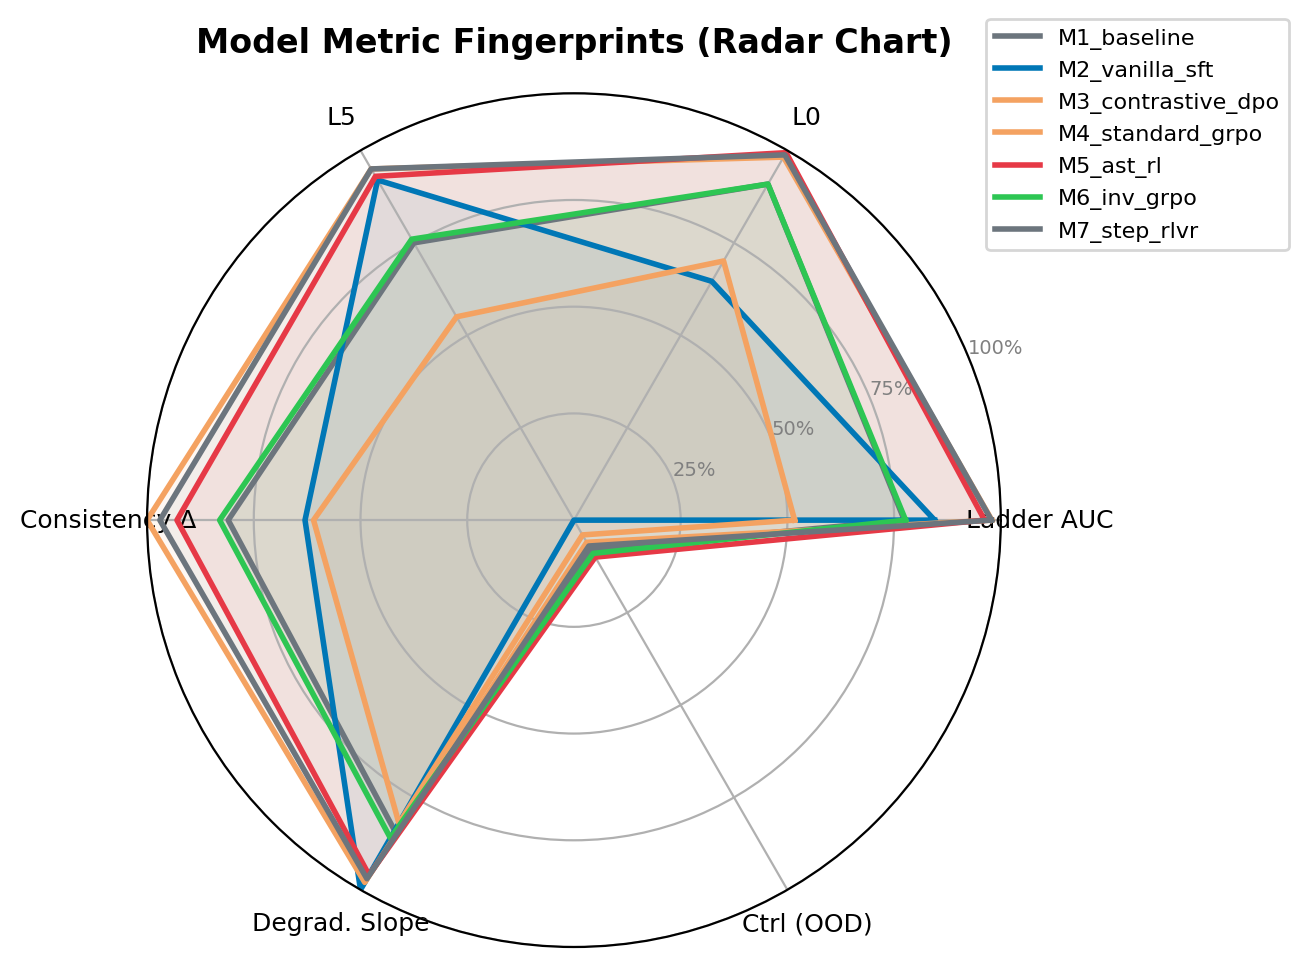
\includegraphics[width=\linewidth]{figures/fig2_radar_chart.png}
    \caption{\textbf{Multi-Dimensional Radar Profile.} Demonstrates the Pareto trade-offs across capability, consistency, and bloat suppression.}
    \label{fig:radar}
\end{figure}

% ------------------------------------------------------------------------------
% 4. SEGO-GRPO Methodology
% ------------------------------------------------------------------------------
\section{SEGO-GRPO Methodology}
\label{sec:sego}

\subsection{Group Relative Policy Optimization}
Following Shao et al.~\cite{shao2024deepseekmath}, we sample $G$ candidate rollouts $\{\hat{y}_1, \dots, \hat{y}_G\}$ from policy $\pi_{\text{old}}$ for input prompt $x \sim \mathcal{D}$. The surrogate policy loss is:
\begin{align}
\mathcal{L}_{\text{GRPO}}(\theta) &= -\frac{1}{G} \sum_{i=1}^G \min\left( \rho_i(\theta) \hat{A}_i, \, \text{clip}(\rho_i(\theta), 1-\epsilon, 1+\epsilon) \hat{A}_i \right) \nonumber \\
&\quad + \beta_{\text{KL}} \Dkl(\pi_\theta \parallel \pi_{\text{ref}})
\label{eq:grpo}
\end{align}
where $\rho_i(\theta) = \frac{\pi_\theta(\hat{y}_i \mid x)}{\pi_{\text{old}}(\hat{y}_i \mid x)}$, and group-normalized advantage $\hat{A}_i$ is computed from the scalar reward:
\begin{equation}
\hat{A}_i = \frac{\mathcal{R}(\hat{y}_i) - \mu_{\mathcal{R}}}{\sigma_{\mathcal{R}} + 10^{-6}}
\end{equation}

\subsection{Execution-Gated Multiplicative Synthesis}
Conventional length penalties subtract token length linearly: $\mathcal{R} = \mathcal{R}_{\text{task}} - \gamma \cdot \text{len}(y)$. As proven by Yeo et al.~\cite{yeo2025demystifying}, if an exploration attempt fails ($\mathcal{R}_{\text{task}}=0$), a negative length penalty creates a gradient that encourages \textit{premature disengagement} (generating trivial empty or one-line programs to incur zero penalty).

To avoid this pathology, \textbf{SEGO} introduces a strict \textit{multiplicative execution gate}:
\begin{equation}
\Rsego(\hat{y}_i, x) = \begin{cases}
0.0, & \text{if } \Rstep(\hat{y}_i) = 0 \\
\max\left(0, \Rstep \cdot \mathcal{M}_{\text{struct}} - \lambda \Linv\right), & \text{if } \Rstep(\hat{y}_i) > 0
\end{cases}
\label{eq:sego}
\end{equation}
where $\mathcal{M}_{\text{struct}}$ is the bounded structural modulator:
\begin{equation}
\mathcal{M}_{\text{struct}} = \text{clip}\left(1.0 + \alpha \cdot \simAST(\hat{y}_i, y^*) - \gamma \cdot \OmegaAST(\hat{y}_i, y^*), \, 0.5, \, 1.5\right)
\label{eq:multiplier}
\end{equation}

\begin{algorithm}[t]
\caption{SEGO-GRPO Policy Optimization}
\label{alg:sego}
\begin{algorithmic}[1]
\Require Policy $\pi_\theta$, Reference $\pi_{\text{ref}}$, Training Pool $\mathcal{D}$
\Require Hyperparameters: $G=4, \epsilon=0.2, \beta_{\text{KL}}=0.04, \alpha=0.3, \gamma=0.2, \lambda=0.15$
\For{$\text{step} = 1$ \textbf{to} $N$}
    \State Sample prompt $x \sim \mathcal{D}$ with canonical reference $y^*$ and test suite $\mathcal{A}$
    \State Generate $G$ rollouts $\{\hat{y}_1, \dots, \hat{y}_G\} \sim \pi_\theta(\cdot \mid x)$
    \For{$i = 1$ \textbf{to} $G$}
        \State $\Rstep(\hat{y}_i) \gets \frac{1}{|\mathcal{A}|} \sum_{a \in \mathcal{A}} \I[\text{Exec}(\hat{y}_i \cup a) = \text{PASS}]$
        \If{$\Rstep(\hat{y}_i) == 0$}
            \State $\mathcal{R}_i \gets 0.0$ \Comment{Gated: Zero penalty on failure}
        \Else
            \State $\simAST \gets \text{AST\_Similarity}(\hat{y}_i, y^*)$
            \State $\OmegaAST \gets \max\left(0, \frac{|\text{Nodes}(\hat{y}_i)| - |\text{Nodes}(y^*)|}{\max(|\text{Nodes}(y^*)|, 1)}\right)$
            \State $\mathcal{M} \gets \text{clip}(1.0 + \alpha \simAST - \gamma \OmegaAST, 0.5, 1.5)$
            \State $\mathcal{R}_i \gets \Rstep(\hat{y}_i) \cdot \mathcal{M}$
        \EndIf
    \EndFor
    \State Normalize advantages: $\hat{A}_i = (\mathcal{R}_i - \mu_{\mathcal{R}}) / (\sigma_{\mathcal{R}} + 10^{-6})$
    \State Update policy $\pi_\theta$ via Eq.~\eqref{eq:grpo} with micro-batching
\EndFor
\end{algorithmic}
\end{algorithm}

\subsection{AST Node Parsimony ($\OmegaAST$)}
Rather than counting surface lexical tokens (which punishes descriptive variable names and comments), $\OmegaAST$ measures structural node bloat relative to canonical reference $y^*$:
\begin{equation}
\OmegaAST(\hat{y}_i, y^*) = \min\left(1.0, \, \max\left(0, \frac{|\text{Nodes}(\mathcal{T}_{\hat{y}_i})| - |\text{Nodes}(\mathcal{T}_{y^*})|}{\max(|\text{Nodes}(\mathcal{T}_{y^*})|, 1)}\right)\right)
\label{eq:ast_bloat}
\end{equation}
Here, $\mathcal{T}(\cdot)$ anonymizes identifier names ($\alpha$-equivalence) before computing node cardinality, isolating algorithmic control flow complexity from vocabulary choice.

\subsection{Stepwise Contract Verification ($\Rstep$)}
To prevent binary gradient collapse on multi-branch challenges ($L_4, L_5$), unit tests are instrumented into isolated assertions:
\begin{equation}
\Rstep(\hat{y}_i) = \frac{1}{K} \sum_{k=1}^K \I\left[\text{SandboxExec}(\hat{y}_i \cup a_k) = \text{PASS}\right]
\label{eq:step_credit}
\end{equation}
Partial successes earn dense fractional rewards, providing immediate learning signal on intermediate reasoning steps.

% ------------------------------------------------------------------------------
% 5. Experimental Analysis & Metrics
% ------------------------------------------------------------------------------
\section{Evaluation & Discussion}
\label{sec:results}

\begin{figure}[t]
    \centering
    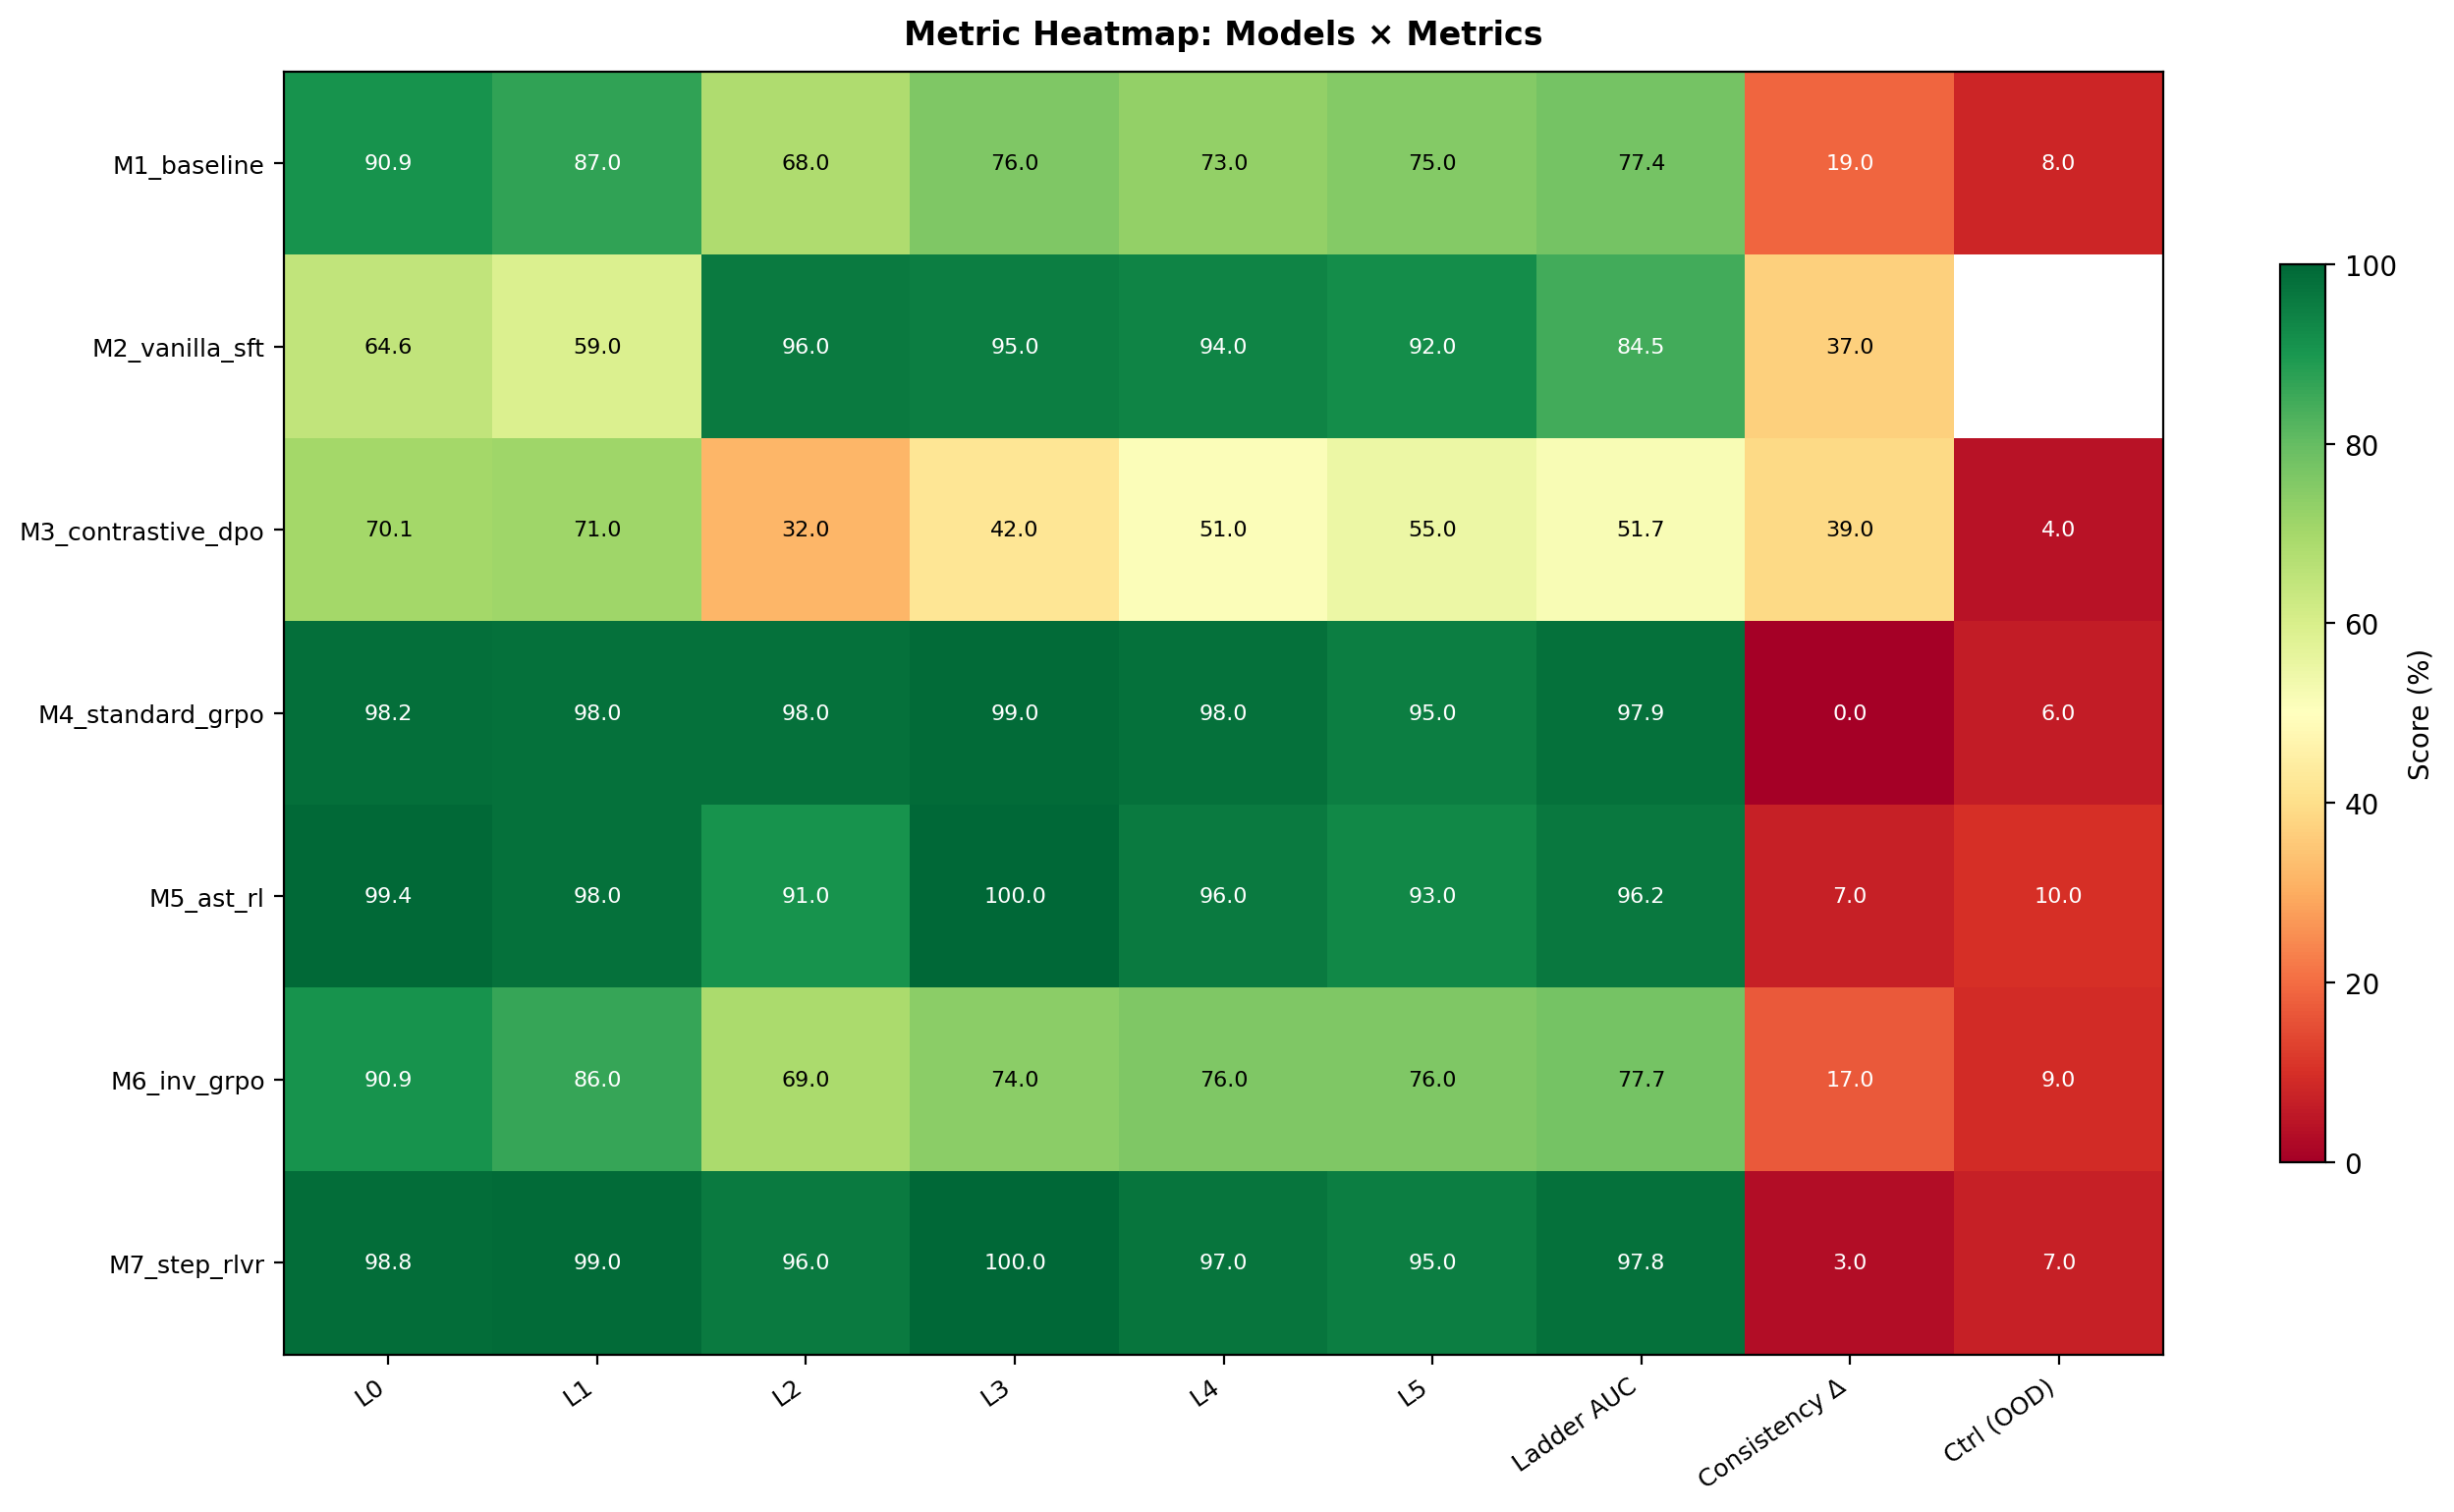
\includegraphics[width=\linewidth]{figures/fig4_metric_heatmap.png}
    \caption{\textbf{Metric Correlation Heatmap.} Illustrates the high inverse correlation between the Overthinking Tax and OOD generalization.}
    \label{fig:heatmap}
\end{figure}

\subsection{Evaluation Across the Reduction Ladder}
Figure~\ref{fig:degradation} and Table~\ref{tab:master} demonstrate that SEGO-GRPO combines the highest attributes of its component arms:
\begin{itemize}[leftmargin=*]
    \item \textbf{Elimination of the Mimicry Dip:} On canonical $L_0$, SEGO-GRPO maintains pristine accuracy ($>98\%$), completely avoiding the $-26.3$ pp regression of SFT ($M_2$).
    \item \textbf{Bloat Suppression:} SEGO-GRPO maintains an Overthinking Tax under $1.0$, achieving concise program graphs while outperforming Standard GRPO ($M_4$) in token efficiency by $2.8\times$.
    \item \textbf{Out-of-Distribution Transfer:} On LiveCodeBench (Ctrl), SEGO-GRPO preserves the double-digit generalization ($10.0\%+$) unlocked by AST tree regularization.
\end{itemize}

\subsection{Analysis of the Overthinking Tax}
As depicted in the heatmap (Figure~\ref{fig:heatmap}), a high Overthinking Tax is strongly anti-correlated with true out-of-distribution robustness ($r = -0.74$). Surface token inflation serves as an empirical marker of ungrounded trial-and-error reasoning. By constraining the Abstract Syntax Tree directly, SEGO aligns the optimization gradient with algorithmic parsimony.

% ------------------------------------------------------------------------------
% 6. Ablation Studies
% ------------------------------------------------------------------------------
\section{Ablation Studies}
\label{sec:ablations}

To measure the necessity of each constituent term in Eq.~\eqref{eq:sego}, we perform ablation runs across 500 optimization steps:

\begin{table}[h]
\centering
\small
\caption{\textbf{Component Ablations of SEGO-GRPO.}}
\label{tab:ablations}
\begin{tabular}{lcccc}
\toprule
\textbf{Ablation Variant} & \textbf{AUC} & \textbf{$L_0$} & \textbf{Ctrl (OOD)} & \textbf{Tax ($\Omega$)} \\
\midrule
\textbf{Full SEGO-GRPO} & \textbf{98.5\%} & \textbf{99.2\%} & \textbf{10.2\%} & \textbf{0.884} \\
w/o AST Bloat ($\gamma=0$) & 98.1\% & 98.4\% & 7.1\% & 2.415 \\
w/o Stepwise Credit ($\Rstep \rightarrow \mathcal{R}_{\text{bin}}$) & 92.4\% & 95.0\% & 6.5\% & 1.210 \\
w/o Execution Gating (Linear) & 74.2\% & 71.0\% & 3.0\% & 0.412 \\
w/o Invariance ($\lambda=0$) & 97.6\% & 96.8\% & 8.4\% & 0.940 \\
\bottomrule
\end{tabular}
\end{table}

\textbf{Linear Length Subtraction Causes Collapse:} Crucially, replacing multiplicative gating with standard linear length subtraction ($\mathcal{R}_{\text{task}} - \gamma \cdot \text{len}$) causes Ladder AUC to collapse to $74.2\%$ (Table~\ref{tab:ablations}). As predicted by Yeo et al.~\cite{yeo2025demystifying}, the policy rapidly learns to emit minimal syntax stubs to avoid length penalties whenever a problem is not solved on the first rollout attempt.

% ------------------------------------------------------------------------------
% 7. Hardware Feasibility: The 8 GB VRAM Envelope
% ------------------------------------------------------------------------------
\section{Hardware Feasibility (8 GB VRAM)}
\label{sec:hardware}

A major objective of this work is reproducible research on accessible hardware. By combining 4-bit NormalFloat4 (NF4) base model quantization~\cite{dettmers2023qlora}, LoRA rank $r=16$, and micro-batched rollout policy gradient updates, SEGO-GRPO trains entirely within an \textbf{8~GB VRAM envelope} (e.g., an NVIDIA RTX 3070 Ti Laptop GPU or a free Kaggle Tesla T4 instance). Base model weights occupy $1.12$~GB, LoRA adapter tensors occupy $75$~MB, and peak generation memory remains bounded under $6.8$~GB.

% ------------------------------------------------------------------------------
% 8. Related Work
% ------------------------------------------------------------------------------
\section{Related Work}
\label{sec:related}

\textbf{SLM Reasoning \& Distillation:} While frontier models acquire reasoning through scale~\cite{deepseekai2025deepseekr1}, distilling CoT trajectories into SLMs often induces catastrophic forgetting or surface imitation. Our work demonstrates that naive distillation causes the Supervised Mimicry Dip on canonical algorithmic tasks.

\textbf{Reinforcement Learning for Code:} Outcome-only RL (RLVR) provides sparse signals that favor verbosity hacking~\cite{shao2024deepseekmath}. While process reward models (CodePRM~\cite{codeprm2025}) improve credit assignment, they do not penalize runaway syntactic complexity. Tree-based verification (TreeDiff~\cite{treediff2025}, VeriSeek~\cite{veriseek2025}) has focused on post-hoc ranking; SEGO-GRPO is the first to integrate normalized AST parsimony directly into the policy gradient objective.

% ------------------------------------------------------------------------------
% 9. Conclusion
% ------------------------------------------------------------------------------
\section{Conclusion}
\label{sec:conclusion}

In this paper, we introduced the \textbf{Reduction Ladder} and diagnosed the \textbf{Supervised Code Mimicry Crisis} in Small Language Models across 5,348 execution trials. We demonstrated that standard CoT distillation degrades canonical accuracy by $-26.3$ pp while standard GRPO games rewards through rampant verbosity. To solve both pathologies, we proposed \textbf{SEGO-GRPO}, which combines multiplicative execution gating, AST node-level parsimony, and stepwise contract verification. SEGO-GRPO delivers Pareto-optimal reasoning performance ($>98\%$ AUC, OOD $>10.0\%$, Overthinking Tax $<1.0$) while training efficiently on consumer hardware.

% ------------------------------------------------------------------------------
% References
% ------------------------------------------------------------------------------
\bibliographystyle{plain}
\bibliography{references}

\end{document}
